\documentclass[12pt]{article}
\usepackage{fullpage,enumitem,amsmath,amssymb,graphicx,grffile,float,listings}



\begin{document}
    %Title Section
    \begin{flushleft}
    \LARGE CS229 Fall 2017\\
    \LARGE Problem Set \#3 Solutions:  Deep Learning \& Unsupervised Learning \\
    \textbf{\normalsize Author: LFhase \quad rimemosa@163.com}
    \end{flushleft} 
    \noindent
    \rule{\linewidth}{0.4pt}
    %Title Section

    %Problem and Solution
    \section*{A Simple Neural Network}
    \begin{enumerate}[label=(\alph*)]
        \item Using Chain Rule, we know that 
        $$\frac{\partial loss}{\partial w_{1,2}^{[1]}}
        = \frac{\partial loss}{\partial o}\frac{\partial o}{\partial h_2}\frac{\partial h_2}{\partial w_{1,2}^{[1]}}$$
        let $g(x)$ denote the sigmoid function, then we have
        $$g'(x) = g(x)(1-g(x))$$
        so $$\frac{\partial loss}{\partial w_{1,2}^{[1]}}
        =\frac{2}{m}\sum_{i=1}^m (o^{(i)}-y^{(i)})o^{(i)}(1-o^{(i)})w_2^{[2]}h_2^{(i)}(1-h_2^{(i)})x^{(i)}_1$$
        where 
        $$h_2^{(i)}=g(x^{(i)}_1w_{1,2}^{[1]}+x^{(i)}_2w_{2,2}^{[1]}+w_{0,2}^{[1]})$$
        \item let $(0.5,0.5)$, $(3.5,0.5)$, $(0.5,3.5)$ be the three poinst of the triangle.
        The forward transport in the neural network can be written in matrix form.
        $$
        \left[\begin{matrix}
            -1.5 & 3 & 0 \\
            -1.5 & 0 & 3 \\
            9 & -3 & 3\\
        \end{matrix}\right] 
        \times
        \left[\begin{matrix}
            1 \\
            x_1 \\
            x_2\\
        \end{matrix}\right]
        $$
        and
        $$
        \left[\begin{matrix}
            -1 & -1 & -1 & 2.33
        \end{matrix}\right] 
        \times
        \left[\begin{matrix}
            1 \\
            h_1 \\
            h_2\\
            h_3\\
        \end{matrix}\right]
        $$
        Once the point is in the triangle, the first product will be 
        $$
        \left[\begin{matrix}
            1 \\
            1 \\
            1 \\
        \end{matrix}\right]
        $$ 
        So the second product will be -0.67 and the final result will be 0.
        Otherwise, the second product will be larger or equal to 0.33 and the final result will be 1.
        \item Using $f(x)=x$ as hidden layer activation function, we can see the neural network as \textbf{a simple neural network without hidden layer},
        who only has the \textbf{convex boundary} and can't deal with the problem described in statement.
    \end{enumerate}

    \section*{EM for MAP estimation}
    The whole process is the same like what discussed in lecture notes. \\
    Firstly, we have log-likelihood:
    \begin{equation*}
        \begin{split}
            l(\theta) &= \sum_{i=1}^m log[\sum_{z^{(i)}}Q_i(z^{(i)})\frac{p(x^{(i)},z^{(i)}|\theta)}{Q_i(z^{(i)})}] + logp(\theta) \\
            &\geq \sum_{i=1}^m \sum_{z^{(i)}}Q_i(z^{(i)})log\frac{p(x^{(i)},z^{(i)}|\theta)}{Q_i(z^{(i)})} + logp(\theta)
        \end{split}
    \end{equation*}
    So if we set$$Q_i(z^{(i)})=p(z^{(i)}|x^{(i)},\theta)$$
    According to Jensen's Inequality, we have
    $$l(\theta)=\sum_{i=1}^m \sum_{z^{(i)}}Q_i(z^{(i)})log\frac{p(x^{(i)},z^{(i)}|\theta)}{Q_i(z^{(i)})} + logp(\theta)$$
    Then we get EM-step as below: \\
    E-step:$$Q_i(z^{(i)})=p(z^{(i)}|x^{(i)},\theta)$$
    M-step:$$\theta={argmax}_{\theta}[\sum_{i=1}^m \sum_{z^{(i)}}Q_i(z^{(i)})log\frac{p(x^{(i)},z^{(i)}|\theta)}{Q_i(z^{(i)})} + logp(\theta)]$$
    In our assumption, the M-step is tractable. Then we have
    \begin{equation*}
        \begin{split}
            l(\theta^{(t+1)}) 
            &\geq \sum_{i=1}^m \sum_{z^{(i)}}Q_i(z^{(i)})log\frac{p(x^{(i)},z^{(i)}|\theta^{(t+1)})}{Q_i(z^{(i)})} + logp(\theta^{(t+1)}) \\
            &\geq \sum_{i=1}^m \sum_{z^{(i)}}Q_i(z^{(i)})log\frac{p(x^{(i)},z^{(i)}|\theta^{(t)})}{Q_i(z^{(i)})} + logp(\theta^{(t)}) \\
            &= l(\theta^{(t)}) 
        \end{split}
    \end{equation*}
    The likelihood will increase monotonically with each iteration of the algorithm.

    \newpage
    \section*{EM application}
    \begin{enumerate}[label=(\alph*)]
        \item \begin{enumerate}[label=(\roman*)]
            \item Since we have $x^{(pr)} = y^{(pr)} + z^{(pr)} + \epsilon^{(pr)}$, then $X\sim N(\mu_p+\nu_r,\sigma^2+\sigma_p^2+\tau_r^2)$
            So the joint distribution have the mean vector and covariance matrix as below:
            $$
            \left[\begin{matrix}
                \mu_p \\
                \nu_r \\
                \mu_p+\nu_r \\
            \end{matrix}\right]
            $$ 
            and
            $$
            \left[\begin{matrix}
                \sigma_p^2  & 0 & \sigma_p^2 \\
                0 & \tau_r^2 & \tau_r^2 \\
                \sigma_p^2 & \tau_r^2 & \sigma^2+\sigma_p^2+\tau_r^2\\
            \end{matrix}\right]
            $$ 
            \item Using the formula in the notes, we have the mean vector and covariance matrix as below:
            $$
            \mu_Q = 
            \left[\begin{matrix}
                \mu_p \\
                \nu_r \\
            \end{matrix}\right]
            +
            \left[\begin{matrix}
                \sigma_p^2 \\
                \tau_r^2 \\
            \end{matrix}\right]\frac{x^{(pr)}-(\mu_p+\nu_r)}{\sigma^2+\sigma_p^2+\tau_r^2}
            $$ 
            and
            $$
            \Sigma_Q = 
            \left[\begin{matrix}
                \sigma_p^2  & 0  \\
                0 & \tau_r^2 \\
            \end{matrix}\right]
            -
            \left[\begin{matrix}
                \sigma_p^2 \\
                \tau_r^2 \\
            \end{matrix}\right]\frac{            
                \left[\begin{matrix}
                    \sigma_p^2 & \tau_r^2
            \end{matrix}\right]}{\sigma^2+\sigma_p^2+\tau_r^2}
            $$
            The expression is:
            $$Q_{pr}(y^{(pr)},z^{(pr)}) = \frac{1}{\sqrt{{2\pi}^2|\Sigma_Q|}}exp(-\frac{1}{2}
            (\left[\begin{matrix}
                y^{(pr)} \\
                z^{(pr)} \\
            \end{matrix}\right]-\mu_Q)^T 
            \Sigma_Q^{-1}
            (\left[\begin{matrix}
                y^{(pr)} \\
                z^{(pr)} \\
            \end{matrix}\right]-\mu_Q)
            )$$
        \end{enumerate}
        \item We want to maxmize the lower bound of the log-likelihood function:
        \begin{equation*}
            \begin{split}
                \Theta &= argmax_\Theta \sum_p \sum_r E_{(y^{(pr)},z^{(pr)})\sim Q_{pr}}[logp(x^{(pr)},y^{(pr)},z^{(pr)})] \\
                &= argmax_\Theta  \sum_p \sum_r E
                [
                    log\frac{1}{{2\pi}^{3/2}\sigma \sigma_p \tau_r}
                    -\frac{1}{2\sigma_p^2}(y^{(pr)}-\mu_p)^2
                    -\frac{1}{2\tau_r^2}(z^{(pr)}-\nu_r)^2\\
                    &-\frac{1}{2\sigma^2}(x^{(pr)}-y^{(pr)}-z^{(pr)})^2
                ]\\
                &=argmax_\Theta  \sum_p \sum_r E
                [
                    log\frac{1}{\sigma_p \tau_r}
                    -\frac{1}{2\sigma_p^2}(y^{(pr)}-\mu_p)^2
                    -\frac{1}{2\tau_r^2}(z^{(pr)}-\nu_r)^2
                ]
            \end{split}
        \end{equation*}
        Then we calculate the derivatives of each parameter and set them to zero to get the update value.
        $$\mu_p = \frac{1}{PR} \sum_p \sum_r {\mu_Q}_1$$
        $$\nu_r = \frac{1}{PR} \sum_p \sum_r {\mu_Q}_2$$
        $$\sigma_p^2 =\frac{1}{PR}\sum_p \sum_r ({\Sigma_Q}_{11}+{\mu_Q}_1^2-2{\mu_Q}_1\mu_p+\mu_p^2) $$
        $$\tau_r^2 =\frac{1}{PR}\sum_p \sum_r ({\Sigma_Q}_{22}+{\mu_Q}_2^2-2{\mu_Q}_2\nu_r+\nu_r^2) $$
    \end{enumerate}

    \section*{KL divergence and Maximum Likelihood}
    \begin{enumerate}[label=(\alph*)]
        \item  
        \begin{equation*}
            \begin{split}
                KL(P||Q) &= \sum_x P(x)-log\frac{Q(X)}{P(X)}\\
                &\geq  -log\sum_x(P(x)\frac{Q(X)}{P(X)})\\
                &= -log\sum_x Q(x)\\
            \end{split}
        \end{equation*}
        Since $\sum_x  Q(x) = 1$, so $KL(P||Q)\geq 0$. \\
        If $P=Q$, it's easily to see that $KL(P||Q)= 0$. \\
        Because $-log(x)$ is a strictly convex function, so we have the $=$ when $X=E[X]$ with probability 1 where $X=\frac{Q}{P}$.
        \item 
        \begin{equation*}
            \begin{split}
                KL(P(X)||Q(X)) + KL(P(Y|X)||Q(Y|X))&= \sum_x P(x) log\frac{P(x)}{Q(x)} + \sum_x P(x)(\sum_yP(y|x)log\frac{P(y|x)}{Q(y|x)})\\
                &=\sum_x P(x) (\sum_yP(y|x)log(\frac{P(x)}{Q(x)} \frac{P(y|x)}{Q(y|x)})\\
                &=\sum_x \sum_y P(x,y) log(\frac{P(y,x)}{Q(y,x)}) \\
                &=KL(P(Y,X)||Q(Y,X))
            \end{split}
        \end{equation*}
        \item 
        \begin{equation*}
            \begin{split}
                KL(\hat{P}||P_{\theta})&= \sum_x \hat{P} log\frac{\hat{P}(x)}{P_\theta (x)} \\
                &= -\sum_x \frac{1}{m} \Sigma_{i=1}^m \boldsymbol{1}\{x^{(i)}=x\} log\frac{P_\theta (x)}{\Sigma_{i=1}^m \boldsymbol{1}\{x^{(i)}=x\}}\\
                &= -\frac{1}{m} \Sigma_{i=1}^m logP_\theta (x^{(i)})
            \end{split}
        \end{equation*}
        So adjust $\theta$ to minmize the KL is equivalent to maxmize the log-likelihood function.
    \end{enumerate}

    \section*{K-means for compression}
    Since we have reduced the number of colors to 16, we only need to store the 16 colors and the location information, 
    which decreses the space we need to store the whole image. \\
    Here is the result of k-means with mandrill-small.
    \begin{figure}[H]
        \centering
        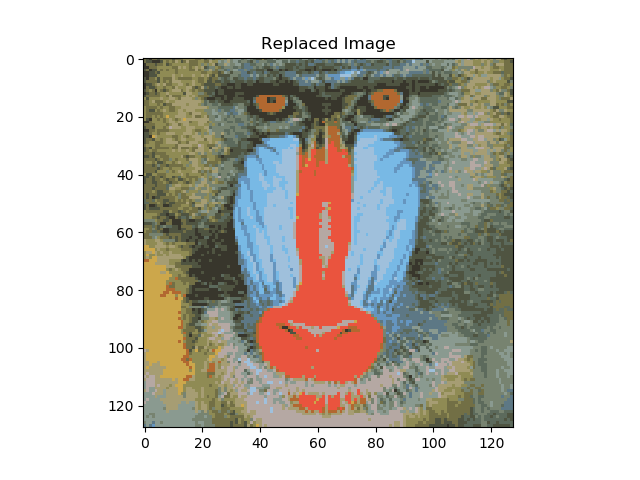
\includegraphics[width=0.80\textwidth]{Q5/replaced_small.png}
    \end{figure}
    \begin{figure}[H]
        \centering
        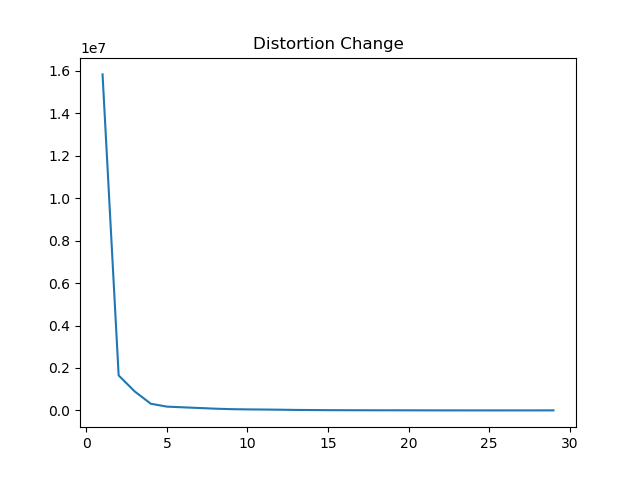
\includegraphics[width=0.60\textwidth]{Q5/distortion_small.png}
    \end{figure}
    \newpage
    Here is the result of k-means with mandrill-large.
    \begin{figure}[H]
        \centering
        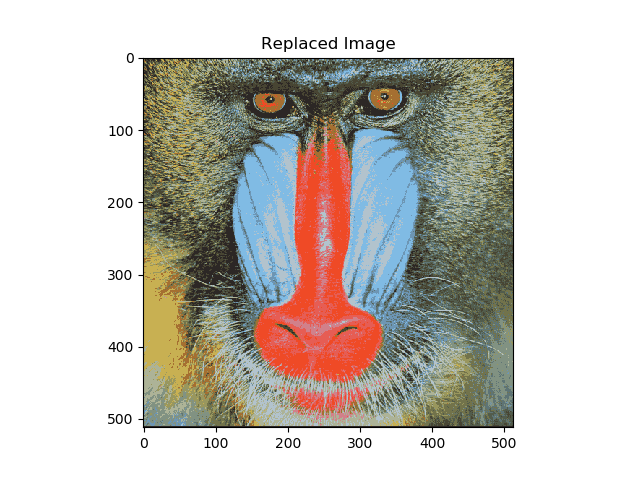
\includegraphics[width=0.80\textwidth]{Q5/replaced_large.png}
    \end{figure}
    \begin{figure}[H]
        \centering
        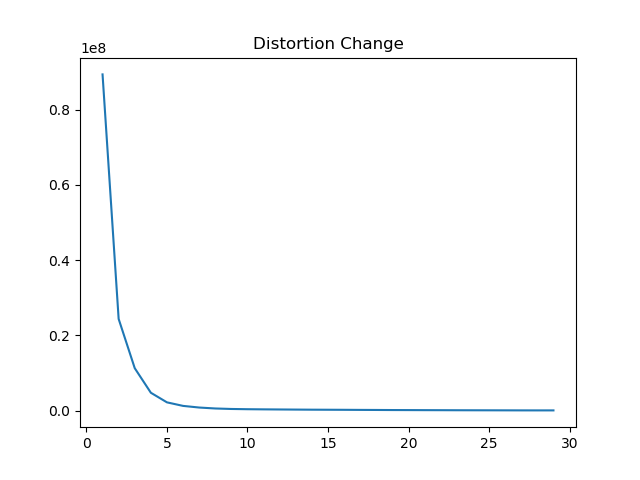
\includegraphics[width=0.60\textwidth]{Q5/distortion_large.png}
    \end{figure}
\end{document}